\usetikzlibrary{arrows,intersections,backgrounds}
\usetikzlibrary{backgrounds}

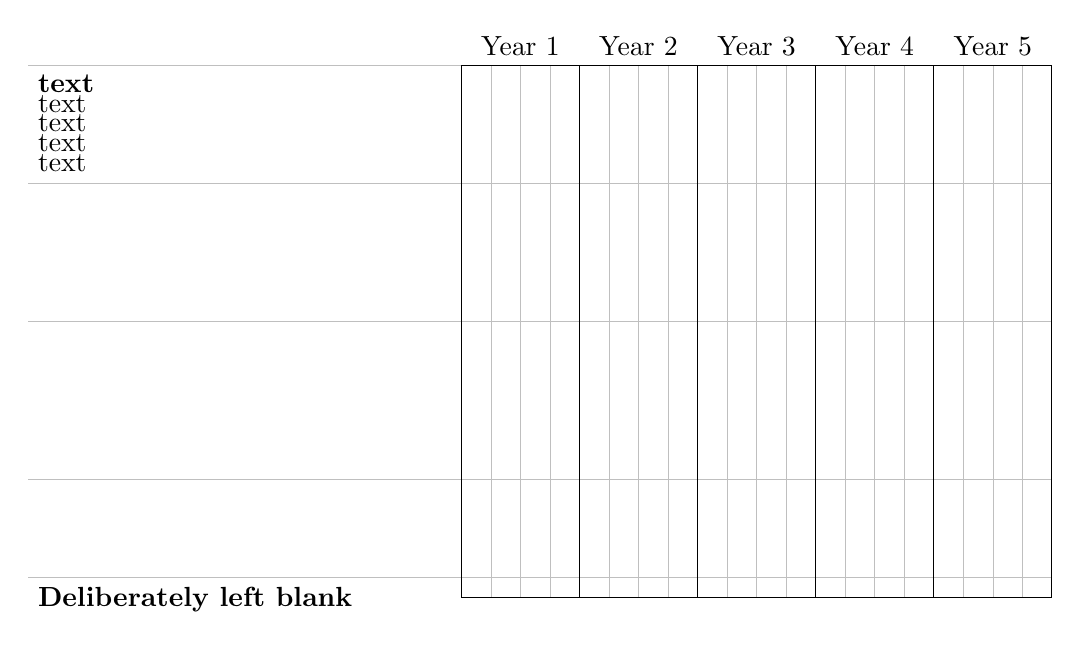
\begin{tikzpicture}[
    scale=.5,
    help lines/.style={
        color=lightgray,
        line width=0.2pt
    }
]

\draw (0,14) node[anchor=north west] {{\bf text}};
\draw (0,13.5) node[anchor=north west] {text};
\draw (0,13) node[anchor=north west] {text};
\draw (0,12.5) node[anchor=north west] {text};
\draw (0,12) node[anchor=north west] {text};


\draw (0,1) node[anchor=north west] {{\bf Deliberately left blank}};

% bounding box
\draw[style=help lines] (11,0.5) rectangle (12.5,14);
\draw[style=help lines] (11.75,0.5) rectangle (13.25,14);
\draw[style=help lines] (14,0.5) rectangle (15.5,14);
\draw[style=help lines] (14.75,0.5) rectangle (16.25,14);
\draw[style=help lines] (17,0.5) rectangle (18.5,14);
\draw[style=help lines] (17.75,0.5) rectangle (19.25,14);
\draw[style=help lines] (20,0.5) rectangle (21.5,14);
\draw[style=help lines] (20.75,0.5) rectangle (22.25,14);
\draw[style=help lines] (23,0.5) rectangle (24.5,14);
\draw[style=help lines] (23.75,0.5) rectangle (25.25,14);

\draw[style=help lines] (0,14) -- (26,14);
\draw[style=help lines] (0,11) -- (26,11);
\draw[style=help lines] (0,7.5) -- (26,7.5);
\draw[style=help lines] (0,3.5) -- (26,3.5);
\draw[style=help lines] (0,1) -- (26,1);
\draw (11,0.5) rectangle (26,14);
\draw (14,0.5) rectangle (23,14);
\draw (17,0.5) rectangle (20,14);

\draw (12.5,14) node[anchor=south] {Year 1};
\draw (15.5,14) node[anchor=south] {Year 2};
\draw (18.5,14) node[anchor=south] {Year 3};
\draw (21.5,14) node[anchor=south] {Year 4};
\draw (24.5,14) node[anchor=south] {Year 5};

% blocks


\end{tikzpicture}